\documentclass[11pt, a4paper, onecolumn, oneside, final]{report}

\usepackage[margin=0.6in, bottom=0.7in]{geometry}
\usepackage{tocbibind}
\usepackage{natbib}
\usepackage{subfig}
\usepackage{float}
\usepackage{booktabs}
\usepackage{multirow}

\usepackage{hyperref}
  \hypersetup{
  	colorlinks=false,
  	pdfborder=0 0 0,
  	linkcolor=blue,
  	citecolor=black,
  	bookmarksopen=false,
  	bookmarksnumbered=true,
  	pdfstartview=FitH,
  	pdfview=FitH
	}
	
\usepackage{url}
  \urlstyle{same}

\usepackage{fancyhdr}

\usepackage{amsmath}
\usepackage{amsfonts}
\usepackage{bm}

\usepackage{listings}
\usepackage{xcolor}
\usepackage{pdfpages}
\usepackage[bahasa]{babel}
\usepackage[fixlanguage]{babelbib}

\definecolor{codegreen}{rgb}{0,0.6,0}
\definecolor{codegray}{rgb}{0.5,0.5,0.5}
\definecolor{codepurple}{rgb}{0.58,0,0.82}
\definecolor{backcolour}{rgb}{0.95,0.95,0.92}

\lstdefinestyle{mystyle}{
    backgroundcolor=\color{backcolour},   
    commentstyle=\color{codegreen},
    keywordstyle=\color{magenta},
    numberstyle=\tiny\color{codegray},
    stringstyle=\color{codepurple},
    basicstyle=\ttfamily\footnotesize,
    breakatwhitespace=false,         
    breaklines=true,                 
    captionpos=b,           
    keepspaces=true,                 
    showspaces=false,                
    showstringspaces=false,
    showtabs=false,                  
    tabsize=2,
    numbers=none
}

\lstset{style=mystyle}

\title{Tugas Kelompok 3\\Aljabar Numerik Kelas A\\Tahun Ajaran 2020/2021}
\author{Eko Julianto Salim, Hocky Yudhiono, Jonathan Nicholas}

\begin{document}
\begin{titlepage}
    \begin{center}\begin{figure}
            \begin{center}
                
\includegraphics[width=2.5cm]{makara.eps}
            \end{center}
        \end{figure}    
        \vspace*{0cm}
        \textbf{
        	UNIVERSITAS INDONESIA\\
        }
        
        \vspace*{1.0cm}
        % judul thesis harus dalam 14pt Times New Roman
        \textbf{Interpolasi, Turunan, dan Integrasi Numerik} \\[1.0cm]

        \vspace*{2.5 cm}    
        % harus dalam 14pt Times New Roman
        \textbf{Laporan Tugas Kelompok 3} \\
        
        \vspace*{3 cm}
        \textbf{Kelompok A09} \\
        % penulis dan npm
        
\begin{table}[H]
        \centering
        \begin{tabular}{c c}
            Eko Julianto Salim & 1906350925\\
            Hocky Yudhiono & 1906285604 \\
            Jonathan Nicholas & 1906293133\\
        \end{tabular}
        \end{table}
        \vspace*{5.0cm}

        % informasi mengenai fakultas dan program studi
        \textbf{
        	FAKULTAS ILMU KOMPUTER\\
        	DEPOK \\
        	MEI 2021
        }
    \end{center}
\end{titlepage}

\section*{Pendahuluan}

Selain membahas masalah matematis dan numerik murni, ada beberapa masalah yang berhubungan dengan \textit{engineering} dan kehidupan sehari-hari yang sangat berkaitan dengan analisis numerik. Salah satunya ialah mendapatkan prediksi dari data-data yang sudah ada. Dalam bidang matematika ini, ada suatu metode yang dinamakan interpolasi atau \textit{interpolation} yang merupakan teknik estimasi atau memperkirakan titik-titik baru, biasanya direpresentasikan dalam bentuk persamaan kurva atas data-data berupa titik-titik diskret yang sudah dimiliki sebelumnya.

Data-data tersebut pada umumnya diperoleh dari eksperimen dan percobaan-percobaan ataupun survei yang diambil. Interpolasi ini sangat berguna untuk memprediksi nilai-nilai yang berada di antara titik-titik yang tidak diketahui ataupun untuk memprediksi nilai-nilai yang berada di luar jangkauan titik-titik tersebut.

Interpolasi ini sangat berpengaruh terhadap perkembangan teknologi yang ada di dunia. Pada umumnya digunakan untuk pengolahan citra dan pengolahan sinyal serta suara. Perangkat lunak yang kita gunakan untuk mengirim pesan, melakukan \textit{video call}, dan belajar secara daring juga membutuhkan teknik interpolasi serta ekstrapolasi ini dalam perkembangannya.

Selain itu, ada pula permasalahan integrasi dan diferensiasi yang sangat berguna dalam masalah-masalah \textit{engineering}, seperti dalam menghitung pusat massa, melakukan prediksi statistik, peluang, dan probabilitas, memperkirakan kebutuhan energi mesin, performa perangkat, dan sebagainya. Perhitungan kalkulus ini umumnya sangat rumit dihitung secara analitik, sehingga dibutuhkan metode numerik dalam penyelesaiannya. Penerapan analisis numerik dalam kalkulus secara tidak kita sadari menjadi fondasi dalam berbagai peralatan elektronik di sekitar kita. 

Dalam proyek ini, kami akan mengeksplorasi lebih jauh tentang statistika penduduk Indonesia berdasarkan data-data sensus penduduk yang diperoleh dari publikasi pemerintah Indonesia. Kami harap dengan adanya proyek ini, kami dapat lebih jauh belajar tentang interpolasi, metode numerik, manfaatnya bagi kesejahteraan bangsa Indonesia, serta penerapannya juga dalam kehidupan sehari-hari.


\section*{Isi}
Untuk referensi pertanyaan dari laporan ini mengikuti dokumen \texttt{TK 3 Analisis Numerik} yang sudah diberikan. 

\subsection*{Soal 1}

Dalam interpolasi polinomial, pada umumnya akan dicari sebuah polinomial $p(x) = a_0 + a_1x + a_2x^2 + \cdots + a_nx^n$, sehingga polinomial tersebut melewati setiap titik-titik yang diberikan. Titik-titik pasangan $(t_i, y_i)$ yang harus dilewati ialah $(1960, 97.02), (1970, 119.21), (1980, 147.49), (1990, 179.38), (2000, 206.26)$, $(2010, 237.63)$, dan $(2020, 270.20)$. Selanjutnya, kita akan mencari koefisien dari $a_i$ untuk $i = 0$ hingga $n$. Dalam kasus ini, $n = 6$. Untuk mencari koefisien ini, dapat disubstitusikan titik-titik $x_i$ untuk $i \in \{0, 1, \dots, 6\}$ dan akan didapatkan sistem persamaan linear dengan $7$ \textit{unknown} dan $7$ persamaan yang harus diselesaikan.

Dalam octave, kita dapat menggunakan \textit{command} \texttt{x = A} \texttt{\char`\\} \texttt{b}. Matriks ini dikenal dengan nama Vandermonde Matrix. Secara umum, dibutuhkan sekitar $\Omega (n^3)$ flops dalam mencari koefisien-koefisiennya. Kemudian untuk mencari \textit{condition number}-nya, dapat dicari nilai dari $||A|| \cdot ||A^{-1}||$. Ingat kembali, \textit{condition number} pada dasarnya mengakprosimasi sensitivitas \textit{input} data $b$ terhadap solusinya $x$. Hal ini karena pada dasarnya untuk mencari solusi, kita harus mencari tahu inversnya. Tentunya, \textit{condition number} yang besar berarti bahwa $A$ ini hampir singular, dan menyebabkan sistem persamaan ini \textit{ill-conditioned}. Disini \textit{condition number} yang dicari menggunakan norm-2. Penggunaan norm yang berbeda \textbf{tidak merubah kecenderungan} ukuran \textit{condition number} (secara relatif pada norm yang sama).

Lebih lanjut lagi polinomial $p(x)$ tidak harus bergantung pada $x$ saja, Dalam kasus ini, definisikan $p_{6}(t)=c_{0} \varphi_{0}(t)+c_{1} \varphi_{1}(t)+\ldots+c_{6} \varphi_{6}(t)$, dengan $c_{i}$ ialah koefisien dari setiap basis-basis yang bebas linear $\varphi_{i}(t)$, selanjutnya, basis tersebut bisa dimodifikasi dengan berbagai nilai yang dapat mempermudah perhitungan, misalnya dengan basis newton, basis lagrange, maupun basis $x^i$ yang merupakan bentuk umum polinomial. Tentu saja, apabila basis ini di-\textit{expand}, akan dihasilkan basis polinomial yang sama berkat adanya sifat bebas linear ini.

\subsubsection*{1A.}

Dalam kasus ini, bisa kita selesaikan persamaan linear $A\vec{x} = \vec{b}$ sebagai berikut.

$$
\begin{bmatrix}
1 & t_1 & t_1^2 & t_1^3 & t_1^4 & t_1^5 & t_1^6 \\
1 & t_2 & t_2^2 & t_2^3 & t_2^4 & t_2^5 & t_2^6 \\
1 & t_3 & t_3^2 & t_3^3 & t_3^4 & t_3^5 & t_3^6 \\
1 & t_4 & t_4^2 & t_4^3 & t_4^4 & t_4^5 & t_4^6 \\
1 & t_5 & t_5^2 & t_5^3 & t_5^4 & t_5^5 & t_5^6 \\
1 & t_6 & t_6^2 & t_6^3 & t_6^4 & t_6^5 & t_6^6 \\
1 & t_7 & t_7^2 & t_7^3 & t_7^4 & t_7^5 & t_7^6 \\
\end{bmatrix} \begin{bmatrix}
a_0\\
a_1\\
a_2\\
a_3\\
a_4\\
a_5\\
a_6\\
\end{bmatrix} = \begin{bmatrix}
y_0\\
y_1\\
y_2\\
y_3\\
y_4\\
y_5\\
y_6\\
\end{bmatrix}
$$

Matriks $A$ untuk basis ini memiliki \textit{condition number} sekitar $2.6151 \times 10^{29}$. Jelas sekali bahwa sangat \textit{ill-conditioned}. Ingat kembali juga bahwa semakin besar nilai mutlak sebuah bilangan riil, maka akan semakin tidak presisi saat direpresentasikan dalam komputer dengan sistem IEEE-754. Diberikan pula warning pada Matlab bahwa Matrix dekat sekali dengan singular sehingga hasil bisa tidak akurat.

Didapatkan vektor koefisien $[-4.7486 \times 10^{12} \quad 1.4323 \times 10^{10} \quad -1.8001 \times 10^{7} \quad 12066 \quad -4.549 \quad 0.00091468$ $-7.663 \times 10^{-8}]^T$. Koefisien ini cukup besar dan menyebabkan ketidakakurasian dalam perhitungannya.

\subsubsection*{1B.}
Matriks $A$ di atas dengan basis $(t - 1970)^i$ sebagai berikut.

$$
\begin{bmatrix}
1 & -10 & 100 & -1000 & 10000 & -1 \times 10^{5} & 1 \times 10^{6} \\
1 & 0 & 0 & 0 & 0 & 0 & 0 \\
1 & 10 & 100 & 1000 & 10000 & 10^{5} & 1 10^{6} \\
1 & 20 & 400 & 8000 & 1.6 \times 10^{5} & 3.2 \times 10^{6} & 6.4 \times 10^{7} \\
1 & 30 & 900 & 27000 & 8.1 \times 10^{5} & 2.43 \times 10^{7} & 7.29 \times 10^{8} \\
1 & 40 & 1600 & 64000 & 2.56 \times 10^{6} & 1.024 \times 10^{8} & 4.096 \times 10^{9} \\
1 & 50 & 2500 & 1.25 \times 10^{5} & 6.25 \times 10^{6} & 3.125 \times 10^{8} & 1.5625 \times 10^{10} 
\end{bmatrix}
$$

Matriks tersebut memiliki \textit{condition number} sekitar $1.632 \times 10^{10}$. Dengan vektor koefisien $[119.21 \quad 2.2085$ $0.063039 \quad 0.0022585 \quad 0.00031823 \quad .9179 \times 10^{-6} \quad 7.6625 \times 10^{-8}]^T$. Vektor koefisien yang dihasilkan tidak sebesar basis yang sebelumnya. Tentunya presisinya akan meningkat.

\subsubsection*{1C.}

$$
\begin{bmatrix}
1 & -50 & 2500 & -1.25 \times 10^{5} & 6.25 \times 10^{6} & -3.125 \times 10^{8} & 1.5625 \times 10^{0} \\
1 & -40 & 1600 & -64000 & 2.56 \times 10^{6} & -1.024 \times 10^{8} & 4.096 \times 10^{9} \\
1 & -30 & 900 & -27000 & 8.1 \times 10^{5} & -2.43 \times 10^{7} & 7.29 \times 10^{8} \\
1 & -20 & 400 & -8000 & 1.6 \times 10^{5} & -3.2 \times 10^{6} & 6.4 \times 10^{7} \\
1 & -10 & 100 & -1000 & 10000 & -1 \times 10^{5} & 1 \times 10^{6} \\
1 & 0 & 0 & 0 & 0 & 0 & 0 \\
1 & 10 & 100 & 1000 & 10000 & 1 \times 10^{5} & 1 \times 10^{6} \\
\end{bmatrix}
$$

Matriks tersebut memiliki \textit{condition number} sekitar $1.632 \times 10^{10}$, mirip seperti basis sebelumnya. Vektor koefisien yang didapat untuk basis ini ialah $[237.63 \quad 3.6969 \quad 0.044131 \quad 0.0040515 \quad 0.00037365$ $9.4721 \times 10^{-6} \quad 7.6625 \times 10^{-8}]^T$.

\subsubsection*{1D.}

$$
\begin{bmatrix}
1 & -1.6667 & 2.7778 & -4.6296 & 7.716 & -12.86 & 21.433 \\
1 & -1.3333 & 1.7778 & -2.3704 & 3.1605 & -4.214 & 5.6187 \\
1 & -1 & 1 & -1 & 1 & -1 & 1 \\
1 & -0.66667 & 0.44444 & -0.2963 & 0.19753 & -0.13169 & 0.087791 \\
1 & -0.33333 & 0.11111 & -0.037037 & 0.012346 & -0.0041152 & 0.0013717 \\
1 & 0 & 0 & 0 & 0 & 0 & 0 \\
1 & 0.33333 & 0.11111 & 0.037037 & 0.012346 & 0.0041152 & 0.0013717 \\
\end{bmatrix}
$$

\textit{Condition number} dari matriksnya ialah $6104.8$. Dibandingkan dengan setiap basis lain yang ada, \textit{condition number} untuk matriks ini bernilai paling kecil (untuk 1-norm, 2-norm, ataupun \textit{infinity} norm). Vektor koefisien untuk basis ini ialah $[237.63 \quad 110.91$ $39.718 \quad -109.39 \quad -302.65 \quad -230.17 \quad -55.86]^T$.

Secara umum, untuk matriks yang memiliki \textit{condition number} yang besar, koefisien yang dihasilkan juga semakin besar, secara teoritis, hal ini dapat menyebabkan adanya ketidakpresisian saat melakukan ekstrapolasi. Meskipun belum \textit{overflow}, bilangan yang sangat besar akan membuat terjadinya akumulasi galat yang besar juga. Hilangnya angka penting dalam proses perhitungan tersebut menyebabkan kurang tepatnya hasil ekstrapolasi.

\subsection*{Soal 2}

Untuk mencari nilai-nilai yang ada, kita dapat menggunakan metode horner. Secara umum kode yang digunakan ialah sebagai berikut.

\begin{figure}[h!]
    \centering
    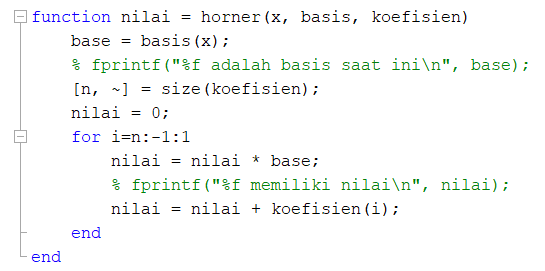
\includegraphics[width=0.5\textwidth]{assets/Horner.png}
    \caption{Potongan Kode Metode Horner untuk Ekstrapolasi}
\end{figure}

Untuk mencari tahu nilai dari suatu polinomial pada suatu titik, dapat kita tuliskan ulang dalam bentuk \textit{nested}-nya. Metode ini secara optimal menghitung nilai dalam kompleksitas $\Omega(N)$.

\begin{figure}[h!]
    \centering
    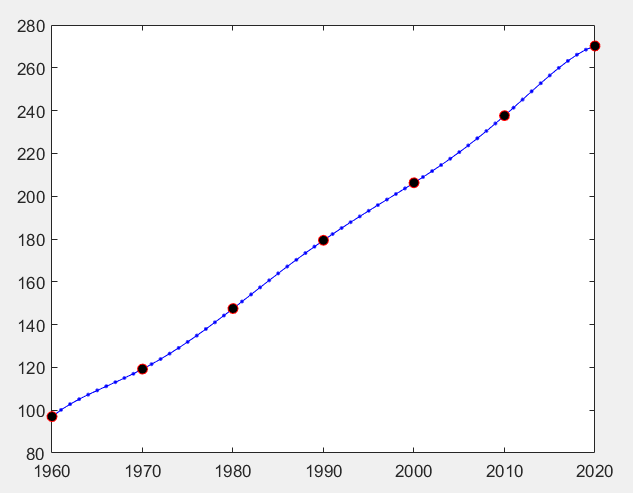
\includegraphics[width=0.5\textwidth]{assets/Plot1.png}
    \caption{Plot Polinomial}
\end{figure}

Secara umum, plot polinomialnya tidak terlalu terlihat bedanya untuk ke setiap basisnya. Untuk basis A, B, C, dan D galat untuk titik-titik yang terinterpolasinya berturut-turut sekitar $0.0179575, 2.9944 \times 10^{-13}, 2.5142 \times 10^{-13}, 4.2276 \times 10^{-13}$.

Menggunakan basis dengan bilangan kondisi terbaik yaitu basis D, didapatkan polinomial $p_6(t)$ sebagai berikut:

\begin{alignat*}{2}
    p_6(t) &= 237.63 + 110.91 (\frac{t - 2010}{30}) + 39.72 (\frac{t - 2010}{30})^2 - 109.39 (\frac{t - 2010}{30})^3 \\
           &\quad- 302.65 (\frac{t - 2010}{30})^4 - 230.17 (\frac{t - 2010}{30})^5 - 55.87 (\frac{t - 2010}{30})^6 \\ 
          &= 237.63 + (\frac{t - 2010}{30}) (110.91 + (\frac{t - 2010}{30}) (39.72 +  (\frac{t - 2010}{30}) (-109.39 + \\ & \quad (\frac{t - 2010}{30}) (-302.65 + (\frac{t - 2010}{30})(-230.17 + (\frac{t - 2010}{30}) (-55.87))))))
\end{alignat*}

\subsection*{Soal 3}

\begin{figure}[h!]
    \centering
    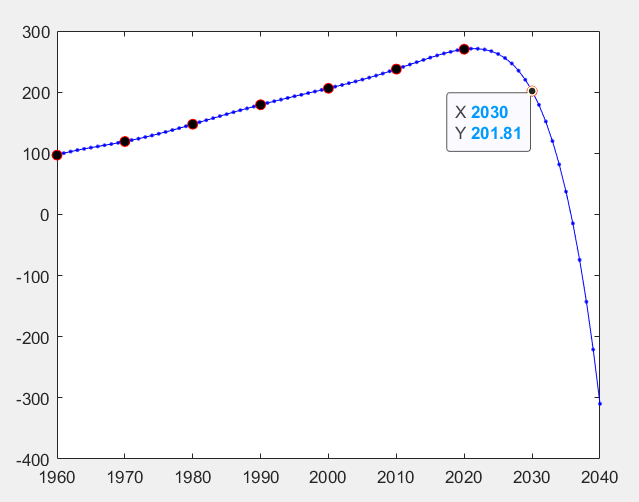
\includegraphics[width=0.45\textwidth]{assets/Plot2.png}
    \caption{Plot Polinomial Hingga Tahun 2040}
\end{figure}

Bila diperhatikan, menggunakan basis pada soal D, didapatkan terdapat sekitar $201.81$ penduduk pada tahun 2030. Selanjutnya, sejak sekitar tahun 2021 sendiri, plotnya mengalami penurunan, tentunya ini jauh sekali dengan perkiraan. \textit{Absolute error}-nya bernilai sekitar $-93.194$ dan \textit{relative error}-nya bernilai sekitar $0.3159$ atau sekitar $31.69\%$.

Hal ini terjadi karena polinomial kita yang memiliki koefisien pada derajat tertingginya bernilai negatif, dan semakin besar derajatnya, bisa terjadi osilasi dan perubahan nilai yang sangat signifikan di ujung-ujung dari polinom. Fenomena ini juga dikenal dengan Runge's Phenomenon. Hasilnya, semakin besar $t$-nya (di luar range awal) maka akan semakin kecil nilainya. Secara umum, polinom ini lebih cocok untuk mengestimasi data yang berada di dalam interval data-data yang diberikan saja (interpolasi), yaitu $[1960, 2020]$.

\subsection*{Soal 4}

Selain menggunakan basis-basis tersebut, akan dicoba juga menggunakan basis newton. Basis newton di sini ialah $\varphi_i(t) = \prod_{k = 0}^{i-1} (t - t_k)$. Basis newton ini tentunya akan menghasilkan polinomial yang sama dengan polinomial pada soal nomor 2, namun apabila kita ingin menambahkan data, kita tidak perlu menghitungnya dari awal, melainkan hanya menambahkan barisan/lapisan koefisien baru sepanjang diagonal terluar. Selanjutnya, kita dapat menggunakan metode \textit{divided difference} dalam mencari koefisien dari polinomial dengan basis ini. 

% \begin{figure}[h!]
%     \centering
%     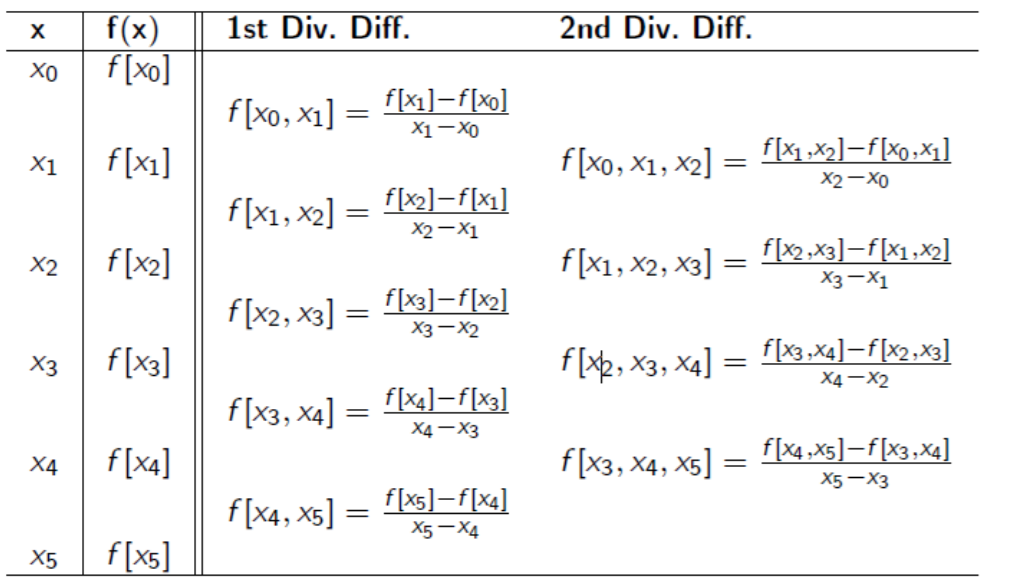
\includegraphics[width=0.6\textwidth]{assets/divDiff.png}
%     \caption{\textit{Divided Difference Table} untuk $n = 5$}
% \end{figure}

Tabel ini pada dasarnya didapatkan dari penjabaran persamaan yang ada. Selanjutnya bila kita ingin menambahkan data, cukup menghitung kembali data-data baru yang mengandung titik data baru tersebut, untuk menambahkan data dari $n$ data yang sudah ada, hanya perlu dilakukan komputasi terhadap $n + 1$ nilai baru dan menambahkan hasil komputasi tersebut pada tabel koefisien \textit{divided difference}.

\begin{figure}[h!]
    \centering
    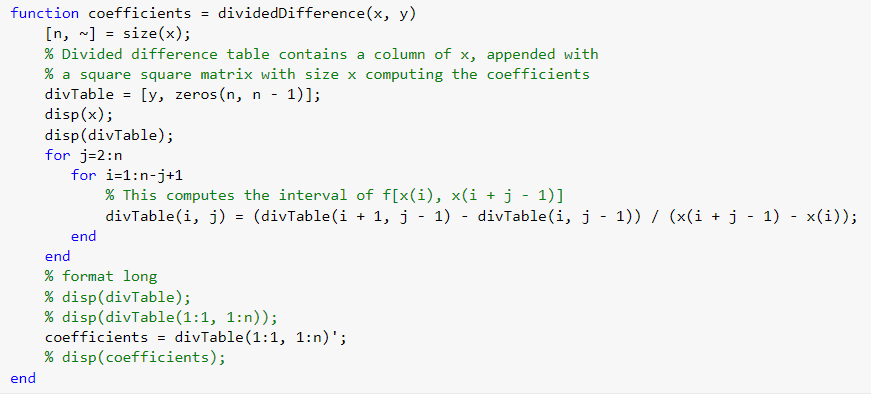
\includegraphics[width=0.6\textwidth]{assets/divided.png}
    \caption{Potongan Kode untuk Mencari Koefisien dari Basis Newton}
\end{figure}

Setelah kita mencari nilai untuk $n = 6$, perhatikan bahwa saat kita menambahkan baris baru, hanya perlu dicari $7$ buah nilai baru, dan akan ditambahkan satu kolom sebagai koefisien untuk basis terakhir yang baru ditambahkan. Nilai-nilai yang sudah ada pada matriks sebelumnya masih bernilai sama dan bisa digunakan kembali.

\begin{figure}[h!]
    \centering
    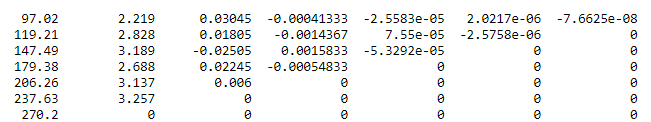
\includegraphics[width=0.8\textwidth]{assets/n6.png}
    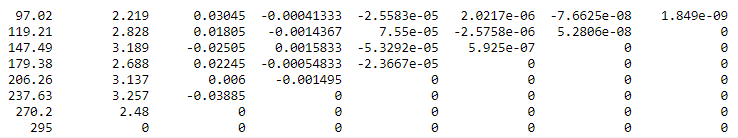
\includegraphics[width=0.8\textwidth]{assets/n7.png}
    \caption{Penambahan Satu Lapis Iterasi Dalam Komputasi}
\end{figure}

Bila kita kembali lakukan \textit{plotting} untuk data yang baru ditambahkan, akan didapatkan grafik sebagai berikut.

\begin{figure}[h!]
    \centering
    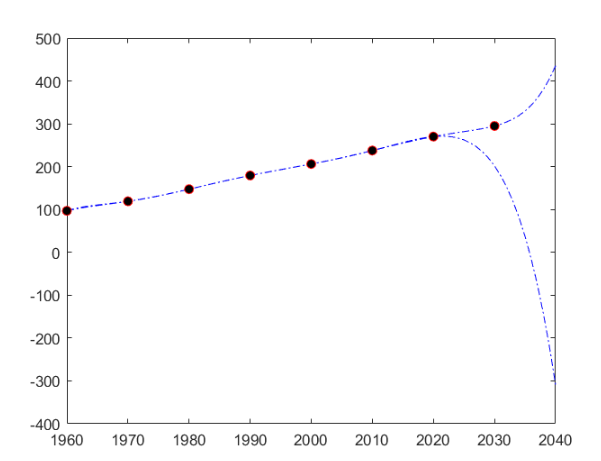
\includegraphics[width=0.5\textwidth]{assets/newtonPlot.png}
    \caption{Plotting dengan Newton untuk Penambahan Data}
\end{figure}

Selanjutnya, kita akan mencoba menginterpolasi data tersebut dengan metode \textit{spline}. Metode ini merupakan salah satu metode yang digunakan untuk meredam derajat polinomial interpolasi agar tidak terjadi \textit{Runge's Phenomenon}. Misalnya pada \textit{linear spline}, data-data tersebut dihubungkan oleh segmen-segmen garis lurus di antara data-data yang diketahui. Untuk melakukan ekstrapolasi atas data-data yang berada di luar interval, biasanya akan digunakan potongan persamaan \textit{spline} terakhir ujung-ujungnya.

\begin{figure}[h!]
    \centering
    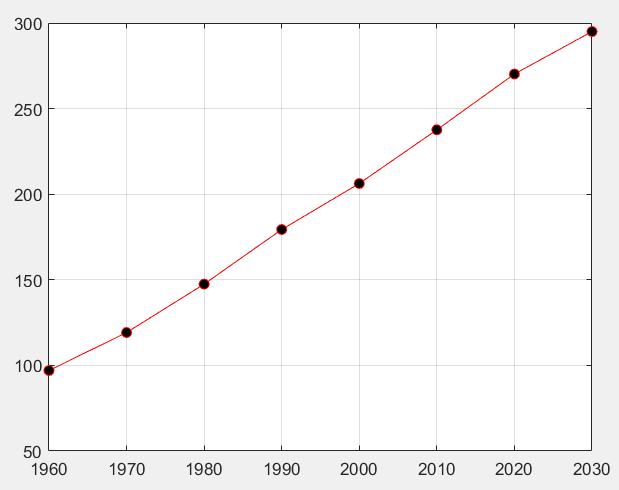
\includegraphics[width=0.4\textwidth]{assets/LinearSpline.png}
    \caption{\textit{Linear Spline}}
\end{figure}

\subsection*{Soal 5}

Selain \textit{linear spline}, pada umumnya digunakan juga \textit{cubic spline}. \textit{Cubic spline} ini memiliki merupakan potongan fungsi-fungsi polinomial derajat 3 yang kontinu tidak hanya pada titik interpolasinya, tapi juga pada turunan pertama dan turunan keduanya.

Apabila diberikan $7$ buah data, maka akan dibuat $6$ buah \textit{spline}, dengan setiap \textit{spline}-nya memiliki properti seperti yang disebutkan di atas. Apabila dihitung, dibutuhkan 2 persamaan lagi agar bisa mendapatkan informasi untuk $6$ buah \textit{spline}. Disini akan digunakan \textit{Natural Cubic Splines}, yang memberikan syarat turunan kedua di kedua ujungnya bernilai 0.

Bila dituliskan secara formal, maka \textit{spline} ke-$i$ ialah $s_i(x) = a_i + b_i(x - x_i) + c_i(x-x_i)^2 + d_i(x-x_i)^3$, untuk $i \in [0, 5]$. Melalui kontribusi nilainya dari persamaan kuadrat, bisa diselesaikan sebuah sistem persamaan linear berbentuk tridiagonal untuk mencari nilai dari $b_i, c_i$ dan $d_i$. Untuk lebih jelasnya bisa dilihat pada program \texttt{no5.m} yang terlampir. Didapatkan sebuah matriks aproksimasi berikut (hanya ditampilkan dalam 5 angka penting) dengan baris ke-$i$ menyatakan spline ke-$i$, dengan kolom pertama hingga kolom keempat berturut-turut menyatakan $a_i, b_i, c_i$ dan $d_i$.

$$
\begin{bmatrix}
97.02 & 2.0935 & -4.4409 \times 10^{-17} & 0.0012548\\
119.21 & 2.47 & 0.037644 & -0.00018397\\
147.49 & 3.1676 & 0.032125 & -0.0029989\\
179.38 & 2.9105 & -0.057842 & 0.0035596\\
206.26 & 2.8215 & 0.048945 & -0.0017394\\
237.63 & 3.2786 & -0.0032362 & 0.00010787\\
\end{bmatrix}
$$

\begin{figure}[h!]
    \centering
    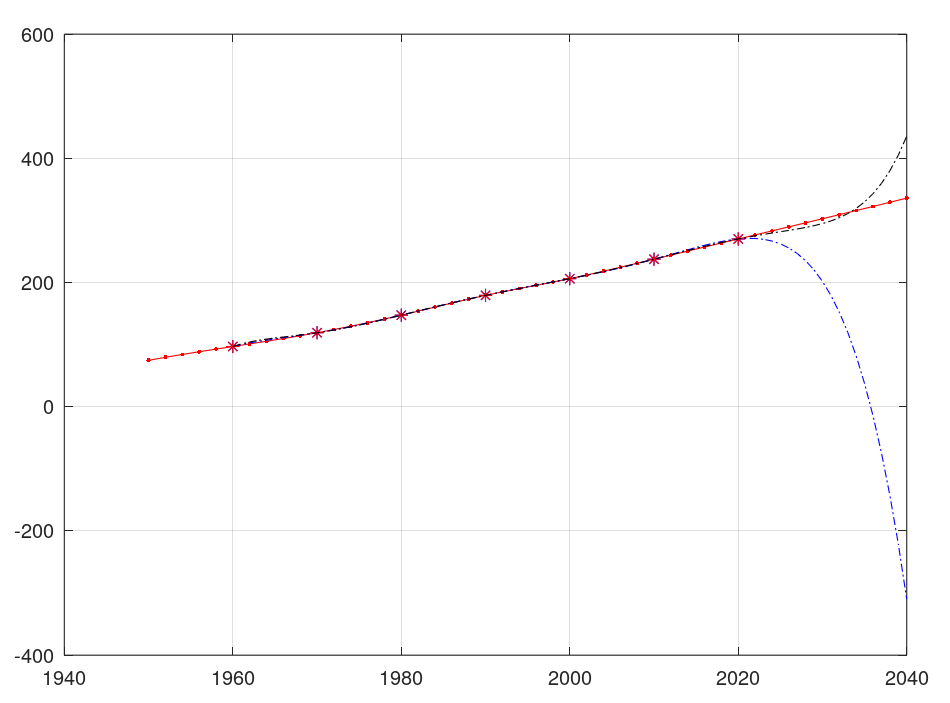
\includegraphics[width=0.75\textwidth]{assets/AllPlot.png}
    \caption{Plot Perbandingan $p_6(t)$, $p_7(t)$, dan \textit{Cubic Splines}}
\end{figure}

Dengan cubic splines, untuk data yang berada di luar interval $[1960, 2020]$ maka akan digunakan splines terluar yang terdekat dengannya, di dalam kasus ini akan digunakan $s_5$, didapatkan nilai pada $x = 2030$ sekitar $296.22$, tentunya nilai ini jauh memprediksi dengan lebih baik dibandingkan dengan interpolasi polinomial kita pada awalnya.

Splines yang ada diplot dan dibandingkan dengan nomor $2$ dan $4$, untuk interval $[1950, 2040]$. Kurva berwarna hitam untuk polinomial dengan basis newton dengan $n = 7$, kurva berwarna biru untuk polinomial dengan $n = 6$. Kurva berwarna merah untuk \textit{cubic spline}s. Dari jauh, tidak terlalu terlihat berbeda. Untuk fungsi ini, memang lebih baik menggunakan \textit{cubic spline} agar tidak terjadi osilasi yang berlebihan untuk memprediksi jumlah penduduk untuk tahun-tahun ke depannya.

\subsection*{Soal 6}

Untuk soal ini, kami akan menggunakan basis newton dalam menghitung nilai dari polinomialnya, dan mencari \textit{error}-nya dengan asumsi \textit{forward error} dari integralnya.

\subsubsection*{Metode Komposit}

Ada beberapa metode yang akan dicoba disini. Yang pertama ada metode trapezoid. Metode ini pada dasarnya membagi beberapa subinterval menjadi beberapa trapesium dan menghitung luasnya. Perhatikan bahwa semakin banyak subintervalnya, maka akan semakin akurat. Secara analitik, dapat ditulis aproksimasinya sebagai $\sum_{i = 1}^N \frac{h}{2}(f(x_i) + f(x_{i - 1}))$ dengan galat $E_N^T = -\frac{f''(\eta)h^2(b-a)}{12}$. 

Ada pula metode komposit simpson yang mengaproksimasinya dengan $\frac{h}{6}(f_0 + f_N + 2 \sum_{i = 1}^{N - 1}f_i + 4 \sum_{i = 1}^N f_{i - \frac{1}{2}}$ dengan galat $O(h^5)$. Diikuti juga dengan metode simpson 3/8, dengan aproksimasi $\frac{3h}{8}(f_0 + f_N + 3 \sum_{i \ne 3k}^{N - 1}f_i + 4 \sum_{i = 1}^{N/3 - 1} f_{3i}$. Pada intinya menggunakan \textit{cubic interpolation}, dan tidak seperti metode simpson biasa yang menggunakan \textit{quadratic interpolation}. Metode ini memiliki galat $O(h^5)$ juga, namun memiliki akurasi dua kali lebih tinggi dari konstanta galatnya yang lebih presisi.

Ada pula metode segi empat atau biasa dikenal dengan \textit{midpoint} dengan mengakprosimasinya sebagai $(x_i - x_{i - 1})f(x_i)$, dengan galat $O(h^2)$. Selanjutnya, didapatkan tabel berikut dalam iterasi dan nilainya.

\begin{table}[h!]
\centering
\begin{tabular}{|c|c|c|c|c|}
\hline
\textbf{Iterasi} & \textbf{Trapezoid} & \textbf{Midpoint} & \textbf{Simpson} & \textbf{Simpson 3/8} \\ \hline
$10$     & $10742.76390911999$ & $10750.83197885250$ & $10748.14262227500$ & $10748.28656613750$ \\ \hline
$100$    & $10748.22956965579$ & $10748.32126414985$ & $10748.29069931851$ & $10748.29071386993$ \\ \hline
$1000$   & $10748.29010224668$ & $10748.29102030297$ & $10748.29071428420$ & $10748.29071428568$ \\ \hline
$10000$  & $10748.29070816528$ & $10748.29071734598$ & $10748.29071428568$ & $10748.29071428567$ \\ \hline
$100000$ & $10748.29071422434$ & $10748.29071431635$ & $10748.29071428589$ & $10748.29071428608$ \\ \hline 
\end{tabular}
\end{table}

Secara berturut-turut bila dibandingkan dengan hasil yang didapatkan saat menggunakan nilai dari hasil integrasi analitiknya, yaitu sekitar $1.0748290714286 \times 10^4$ didapatkan kurva galat sebagai berikut.

\begin{figure}[h!]
    \centering
    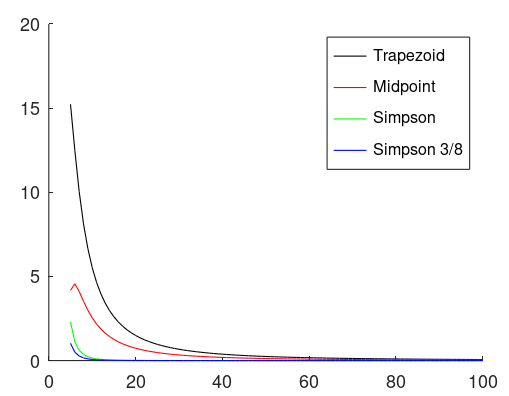
\includegraphics[width=0.45\textwidth]{assets/PlotError.png}
    \caption{Plot Galat dari Setiap \textit{Composite Method}}
\end{figure}

Untuk kompleksitasnya, semua \textit{composite method} bernilai sama, yaitu $\Omega(n)$ untuk banyak subinterval $n$. Untuk pemanggilan fungsi tergantung implementasi, apabila diasumsikan bahwa subinterval metode simpson harus dikalikan 2, maka pemanggilan fungsinya akan dua kali lipat lebih banyak, begitu pula dengan simpson 3/8 akan menjadi tiga kali lebih banyak. Namun secara umum, metode simpson disini sudah sangat baik dengan orde akurasi galat yang sangat cepat menurunnya dan pemanggilan fungsi yang dibutuhkan tidak terlalu banyak.

\subsubsection*{Adaptive Quadrature}

Metode adaptive quadrature ini pada dasarnya mencari aproksimasi integral dengan melakukan rekursi untuk setiap potongan interval selama toleransi yang diinginkan belum tercapai. Adaptive Quadrature sendiri implementasinya beragam, ada yang menggunakan simpson's \textit{method} ataupun \textit{trapezoidal}. Untuk toleransi $10^{-4}$ dengan \textit{trapezoidal method}, dibutuhkan sekitar $15533$ pemanggilan fungsi. Hal ini tidak terlalu efektif bila dibandingkan dengan iterasi biasa. Karena adanya pemanggilan rekursi yang cukup banyak juga menyebabkan \textit{stack memory} meningkat, sehingga metode ini lebih baik digunakan saat kita ingin mendapatkan nilai dengan suatu toleransi tertentu tanpa memperhatikan banyak iterasi yang dibatasi.

\subsubsection*{Romberg Integration}

Pada dasarnya romberg integration ini mengurangi galat berdasarkan berbagai perhitungan \textit{trapezoidal method} dalam sub-interval $2^n$. Setiap iterasinya akan dihitung nilai aproksimasi baru dari rerata yang sudah diberikan bobot, sehingga hasil perhitungan iterasi selanjutnya memiliki galat lebih kecil. Error untuk nilai pada $R_{n, n}$ memiliki orde $O(h^{2n + 2})$. Kompleksitas waktunya ialah $O(2^n + n^2)$. Berikut ialah plot error yang dihasilkan. Untuk $n = 4$, error yang dihasilkan sudah sangat kecil, yaitu $6.2028 \times 10^{-10}$. Bila dibandingkan dengan metode yang lain, metode numerik ini sangat bagus, dan menurut kami yang terbaik dalam mencari nilai aproksimasi integral numerik.

\begin{figure}[h!]
    \centering
    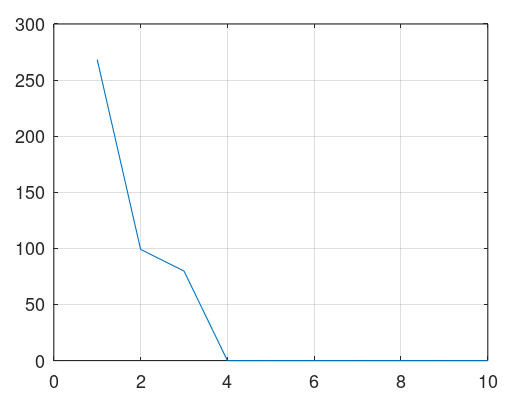
\includegraphics[width=0.3\textwidth]{assets/RombergError.png}
    \caption{Plot Galat dari Romberg Integration}
\end{figure}

\section*{Kesimpulan}

Berbagai metode numerik dalam interpolasi dan integrasi yang ada tentunya memiliki banyak keuntungan dan kerugiannya masing-masing. Ada berbagai metode numerik yang bagus untuk permasalahan tertentu, misalnya dalam melakukan interpolasi polinomial, metode newton sangat baik dalam mengaproksimasi nilai-nilai yang ada di dalam suatu interval, namun bisa terjadi osilasi yang menyebabkan nilai yang berada di luar interval menjadi sangat sensitif. Ada pula metode \textit{cubic spline} yang berusaha menekan sensitivitas ini dengan mempertahankan polinomialnya dalam orde 3, namun memanfaatkan potongan-potongan fungsi di setiap sub-interval dalam mencari nilai aproksimasinya.

Selain itu, dalam integrasi numerik ada pula berbagai metode dengan tujuan yang berbeda. Misalnya ada metode \textit{adaptive quadrature} yang berusaha mengefisiensikan perhitungan sehingga meminimalisir komputasi agar didapatkan toleransi yang diinginkan. Terlepas dari hal ini, bisa juga digunakan metode iterasi biasa, ataupun metode romberg yang membuat aproksimasi lebih baik dari setiap iterasinya.

Pembelajaran yang dilakukan secara lengkap pada metode numerik ini kami rasa merupakan bekal untuk ke depannya agar kami pun dapat mengembangkan suatu metode numerik berkat dari pemikiran kritis dan dasar materi yang kuat.

\nocite{*}
\bibliographystyle{apalike}
\bibliography{bibliography.bib}
\pagenumbering{gobble}
\end{document}